

\subsection{Génération de la carte}
    Pour ce projet nous voulions créer un outil pour créer une carte procéduralement. Pour cela nous avons écrit un programme en C++ qui crée un fichier .OBJ a partir de cartes de bruits.
    \paragraph{Cartes de bruits}
    Une carte de bruit, ou "noisemap", dans le contexte de la génération procédurale, est une technique utilisée pour créer des textures, des terrains ou des environnements de manière algorithmique. Les noisemaps dans la génération procédurale sont utilisées pour introduire des variations naturelles et réalistes dans les modèles générés par ordinateur.
    
    La génération d'une noisemap implique l'utilisation de fonctions de bruit, telles que le bruit de Perlin, le bruit de Simplex ou d'autres algorithmes de bruit procédural. Ces fonctions génèrent des valeurs pseudo-aléatoires qui varient de manière continue et douce à travers l'espace. L'utilisation la plus elementaire de ce genre de cartes et de lier l'élévation du terrain aux valeurs de la carte de bruit.

    \begin{figure}[!h]
        \centering
            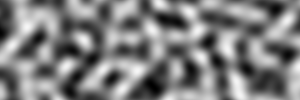
\includegraphics[width=0.5\linewidth]{images/render-noise.png}
            \caption{Visualisation de Carte de bruit}
            \label{fig:enter-label}
    \end{figure}

    Nous pouvons manipuler l'aléatoire des fonctions qui generent ce genre de carte grace a differents parametres:
    \begin{itemize}
        \item La fréquence dans le contexte des fonctions de bruit, comme le bruit de Perlin, détermine la granularité ou la finesse des détails dans la carte de bruit générée. Une fréquence élevée signifie que les variations de bruit se produisent plus rapidement, ce qui entraîne des détails plus fins et plus nombreux dans la carte. À l'inverse, une fréquence basse produit des variations plus lentes et plus douces, résultant en des caractéristiques plus larges et moins détaillées.
        \item Les octaves sont utilisées pour ajouter de la complexité et du réalisme aux cartes de bruit. Chaque octave est une couche supplémentaire de bruit générée à une fréquence différente. En superposant plusieurs octaves, on peut créer des textures plus riches et plus variées. Les octaves sont généralement ajoutées avec des fréquences de plus en plus élevées et des amplitudes de plus en plus faibles.
    \end{itemize}

    \paragraph{Effet sur la Carte Générée}
    \begin{itemize}
        \item \textit{Fréquence Basse} : Une fréquence basse produit des caractéristiques larges et douces. Par exemple, dans la génération de terrains, une fréquence basse peut créer des collines et des vallées larges et douces.
        \item \textit{Fréquence Élevée} : Une fréquence élevée produit des détails fins et nombreux. Par exemple, dans la génération de terrains, une fréquence élevée peut ajouter des rochers, des crevasses et d'autres détails fins à la surface.
        \item \textit{Octaves Multiples} : L'utilisation de plusieurs octaves permet de combiner des caractéristiques larges et douces avec des détails fins. Par exemple, une première octave avec une fréquence basse peut créer les grandes formes du terrain, tandis que des octaves supplémentaires avec des fréquences plus élevées ajoutent des détails fins comme des rochers et des textures de surface.
    \end{itemize}
    \newpage
    Voici des exemples en images de la différence.

    \begin{figure}[!h]
    \centering
    \begin{subfigure}{0.4\linewidth}
        \centering
        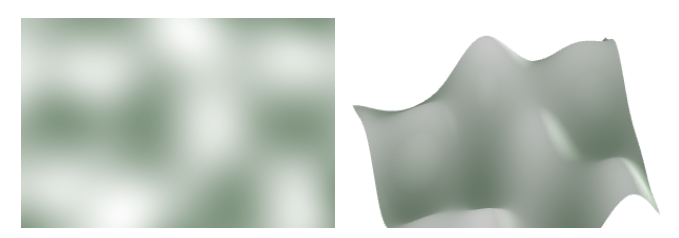
\includegraphics[width=\linewidth]{images/low_frequency.png}
        \caption{Exemple carte et élévation avec une fréquence basse}
        \label{fig:image_avant_expansion}image
    \end{subfigure}
    \hfill
    \begin{subfigure}{0.4\linewidth}
        \centering
        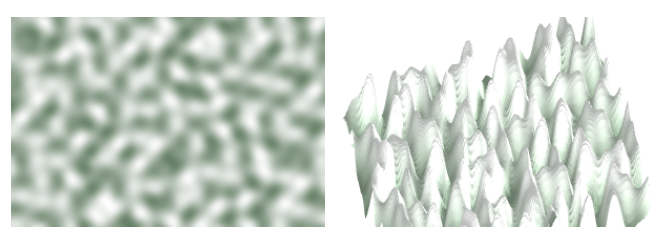
\includegraphics[width=\linewidth]{images/hight_frequency.png}
        \caption{Exemple carte et élévation avec une haute fréquence}
        \label{fig:histo_avant_expansion}
    \end{subfigure}
    \caption{Comparaison de niveau de fréquences}
\end{figure}

    \paragraph{Génération de biomes}
    Sur notre carte nous voulons différents biomes c'est a dire différents environnements repartiimages le plus naturellement possible. Pour cela en plus de la carte de bruit qui va gérer l'élévation du terrain nous allons générer une autre carte de bruit qui va simuler l’humidité du milieux. En combinant ces deux cartes on peut obtenir des biomes plutôt cohérents. En plus de cela nous pouvons définir une élévation minimale qui va permettre de créer des océans.

    Enfin nous avons défini une aire de jeu circulaire au milieu de la carte celle ci sera plate mais utilise quand même les noisemap pour gérer les biomes.


    \begin{figure}[!h]
        \centering
        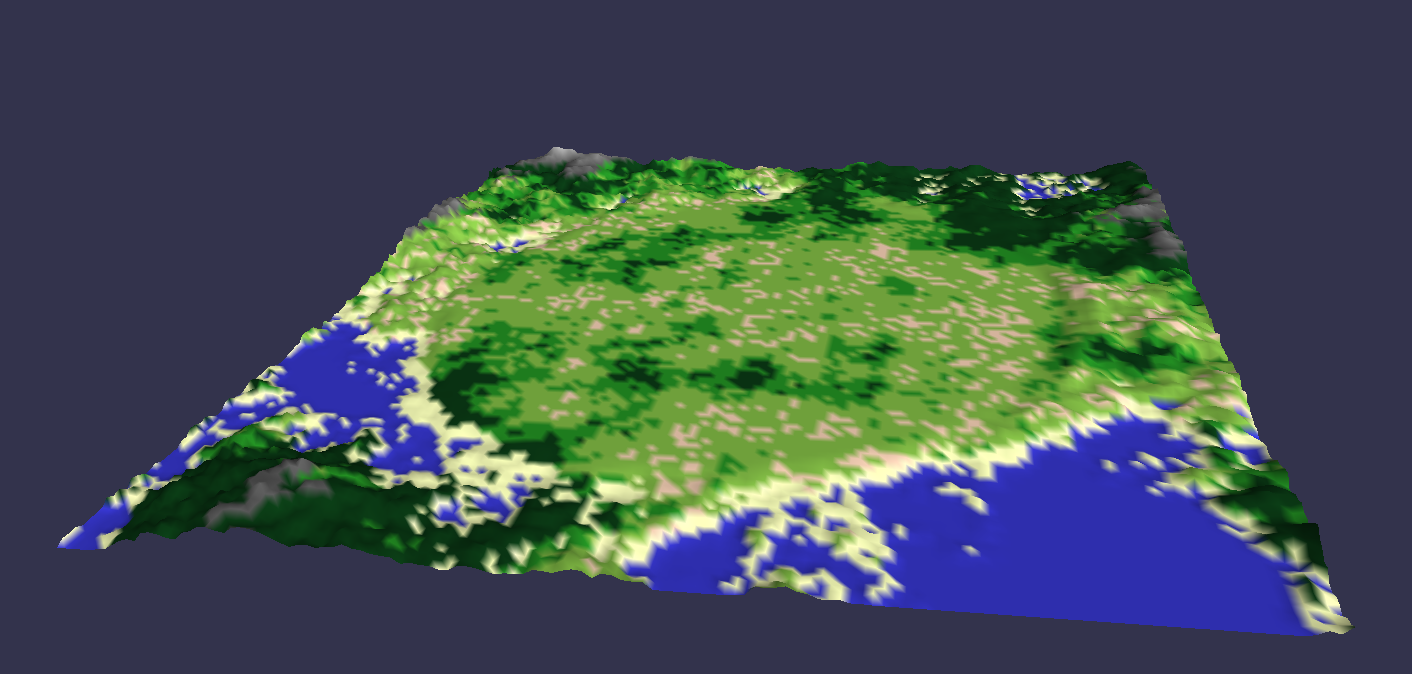
\includegraphics[width=0.5\linewidth]{images/map.png}
        \caption{Une carte générée avec notre code}
        \label{fig:enter-label}
    \end{figure}

    \paragraph{Placer des ressources}
    Un autre défi de la création de la carte est de placer des ressources sur la carte en favorisant les potentielles interaction entre les royaumes, c'est a dire créer des ressources qui serons rares et ne pas les répartir de manière uniformes pour obliger les royaumes a interagir entre eux. Si on prend simplement des positions aléatoires sur la carte par exemple on se retrouve avec un résultat trop uniforme on aimerait avoir une génération avec des trous et des endroits plus concentrés. La solution que nous avons trouvé pour cela ce sont les "Jittered grid" on peut traduire cela par "grille perturbée". Le principe est de générer une grille carrée ou hexagonales et d'appliquer une perturbation aux points de la grille. Voici le résultat.

\begin{figure}[!h]
    \centering
    \begin{subfigure}{0.4\linewidth}
        \centering
        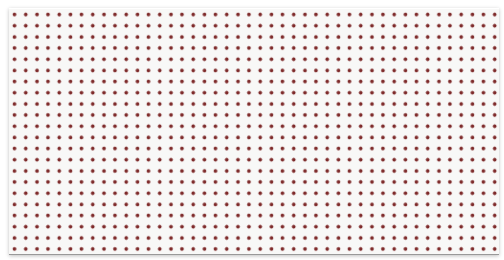
\includegraphics[width=\linewidth]{images/grille.png}
        \caption{Grille avant la perturbation}
        \label{fig:image_avant_expansion}
    \end{subfigure}
    \hfill
    \begin{subfigure}{0.4\linewidth}
        \centering
        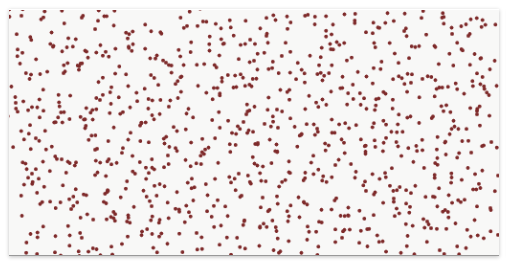
\includegraphics[width=\linewidth]{images/jitter.png}
        \caption{Gille après la perturbation}
        \label{fig:histo_avant_expansion}
    \end{subfigure}
    \caption{Visualisation de jittered grid}
\end{figure}

On voit apparaître des zones avec peu de points et d'autres avec beaucoup de points.

\paragraph{Résultat sur la carte}
Les triangles violets représentent les positions des ressources.
\begin{figure}[!h]
    \centering
    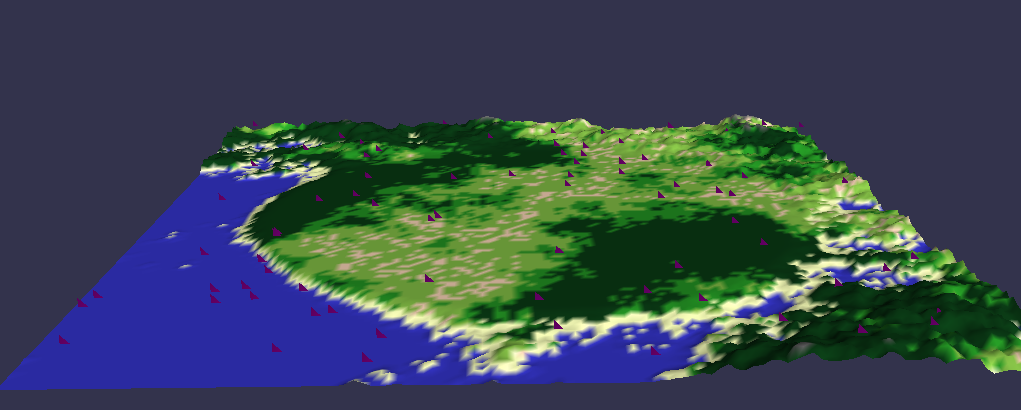
\includegraphics[width=0.5\linewidth]{images/mapjitter.png}
    \caption{Carte avec position de ressources générés}
    \label{fig:enter-label}
\end{figure}

Il suffira de re-exécuter ce code le même nombre de fois que de ressources.